\documentclass[12pt,letterpaper]{article}
\usepackage[english]{babel}
\usepackage[utf8x]{inputenc}
\usepackage{amsmath}
\usepackage{graphicx}
\usepackage[colorinlistoftodos]{todonotes}
\usepackage[top=1in, bottom=1in, left=1in, right=1in]{geometry}
\usepackage{cite}

\begin{document}

\begin{titlepage}

\newcommand{\HRule}{\rule{\linewidth}{0.5mm}} % Defines a new command for the horizontal lines, change thickness here

\center % Center everything on the page
 
%----------------------------------------------------------------------------------------
%   HEADING SECTIONS
%----------------------------------------------------------------------------------------

\textsc{\LARGE University of Tennessee}\\[1.5cm] % Name of your university/college
\textsc{\Large Multivariate Data Mining and Techniques}\\[0.5cm] % Major heading such as course name
\textsc{\large BZAN 552}\\[0.5cm] % Minor heading such as course title

%----------------------------------------------------------------------------------------
%   TITLE SECTION
%----------------------------------------------------------------------------------------

\HRule \\[0.4cm]
{ \huge \bfseries Predict Physical and Chemical Properties of Soil using Spectral Measurements}\\[0.4cm] % Title of your document
\HRule \\[1.5cm]
 
%----------------------------------------------------------------------------------------
%   AUTHOR SECTION
%----------------------------------------------------------------------------------------

% If you don't want a supervisor, uncomment the two lines below and remove the section above
\Large \emph{Author:}\\
Agara Mallesh, Dhanush\\ % Your name
Asudegi, Mohammad Ali\\
Zokaeinikoo, Maryam\\[3cm] % Your name


%----------------------------------------------------------------------------------------
%   DATE SECTION
%----------------------------------------------------------------------------------------

{\large \today}\\[2cm] % Date, change the \today to a set date if you want to be precise

%----------------------------------------------------------------------------------------
%   LOGO SECTION
%----------------------------------------------------------------------------------------


\includegraphics[width=1in]{logo.png}\\[1cm] % Include a department/university logo - this will require the graphicx package
 
%----------------------------------------------------------------------------------------

\vfill % Fill the rest of the page with whitespace

\end{titlepage}


\section{Introduction}
There is an increasingly interest for using infrared spectroscopy for predicting soil functional properties at unsampled locations and to provide data for digital soil mapping \cite{kuang20124}. This technique provides a highly repeatable, rapid and low cost measurement of many soil functional properties \cite{viscarra2009improved}, is non-destructive, no harmful chemicals are used, and importantly, several soil properties can be measured from a single scan \cite{viscarra2006visible}. Therefore, one spectrum can be related to various soil constituents by the multi-parameter feature of this technique.

The diffuse reflectance spectroscopy technique is largely general, quite weak and broad due to overlapping absorptions of soil constituents and their often small concentrations in soil. Therefore, the information needs to be mathematically extracted from the spectra so that they may be correlated with soil properties. Therefore, the analysis of soil diffuse reflectance spectra requires the use of multivariate calibration \cite{martens1989multivariate}. In these cases, to be useful quantitatively, spectra must be related to a set of known reference samples through a calibration model. The set of reference samples used in the models need to be representative of the range of soils in which the models are to be used. Partial least squares regression (PLSR) is the most common algorithm used to calibrate spectra to soil properties \cite{wold1983multivariate}. However, other approaches have also been used, for example, stepwise multiple linear regression \cite{dalal1986simultaneous}, principal components regression (PCR) \cite{chang2001near}, artificial neural networks (ANN) \cite{daniel2003artificial}, multivariate adaptive regression splines (MARS) \cite{shepherd2002development}, boosted regression trees \cite{brown2006global}, PLSR with bootstrap aggregation (bagging--PLSR) \cite{viscarra2007robust}, support vector machines SVM and penalized spline signal regression \cite{stevens2008laboratory}.


\section{Dataset}
The data was ordered in the training and test set. In order to assemble the data, the spatially stratified multilevel sampling design was used. The 60, 10 × 10 km sized “Sentinel Landscapes” was chosen excluding true desserts and areas due to security reasons.

The ultimate goal was to obtain a representative multilevel/multistage sample consisting of:
\begin{itemize}
	\item 60 Sentinel Landscapes
	\item 16 Sampling Clusters per Sentinel Landscape
	\item 10 Sampling Plots per Sampling Cluster
	\item 2 composite Soil samples (topsoil and subsoil) per Sampling Plot
\end{itemize}

Since some locations were either completely inaccessible by four wheeled drive vehicle and on foot or that had soil depth limitations, the actual total number of soil samples is smaller than planned in this dataset.

All samples are characterized with the MIR spectral measurements. The potential spatial predictors, were obtained from NASA remote sensing data missions.

A 10 percent subsample of all the soils went on to be specified with more reference measurements.

Since reference measurements are too expensive (potentially hundreds of US dollars per sample) and tedious, the other 90 percent of samples have been physically archived for calibrating new analytical methods and/or validating old methods.

This research consists of spectral and reference datasets. The training and test data have been split along Sentinel Landscape levels because we are primarily interested in predicting soil properties at new Sentinel Landscapes.

\subsection{Definition of Variables}

Each soil sample has a unique identifier--PIDN. We have 5 response variable to predict and 3587 explanatory variables.\\  

\noindent Response Variables
\begin{itemize}
	\item SOC: Soil organic carbon
	\item pH: pH values
	\item Ca: Mehlich-3 extractable Calcium
	\item P: Mehlich-3 extractable Phosphorus
	\item Sand: Sand content
\end{itemize}

Explanatory Variables:
\begin{itemize}
	\item m7497.96 - m599.76: There are 3,578 mid-infrared absorbance measurements. 
	\item Depth: Depth of the soil sample (2 categories: "Topsoil", "Subsoil")
	\item BSA: average long-term Black Sky Albedo measurements from MODIS satellite images (BSAN = near-infrared, BSAS = shortwave, BSAV = visible)
	\item CTI: compound topographic index calculated from Shuttle Radar Topography Mission elevation data
	\item ELEV: Shuttle Radar Topography Mission elevation data
	\item EVI: average long-term Enhanced Vegetation Index from MODIS satellite images.
	\item LST: average long-term Land Surface Temperatures from MODIS satellite images (LSTD = day time temperature, LSTN = night time temperature)
	\item Ref: average long-term Reflectance measurements from MODIS satellite images (Ref1 = blue, Ref2 = red, Ref3 = near-infrared, Ref7 = mid-infrared)
	\item Reli: topographic Relief calculated from Shuttle Radar Topography mission elevation data
	\item TMAP and TMFI: average long-term Tropical Rainfall Monitoring Mission data (TMAP = mean annual precipitation, TMFI = modified Fournier index)
\end{itemize}

\section{Visualization of Variables}

In first step the visualization of a random number of observations helped to compare the effect of removing CO2 related spectrums, suggested by the Kaggle, also the difference between top soil and subsoil samples.

\begin{figure}[h!]
	\centering
	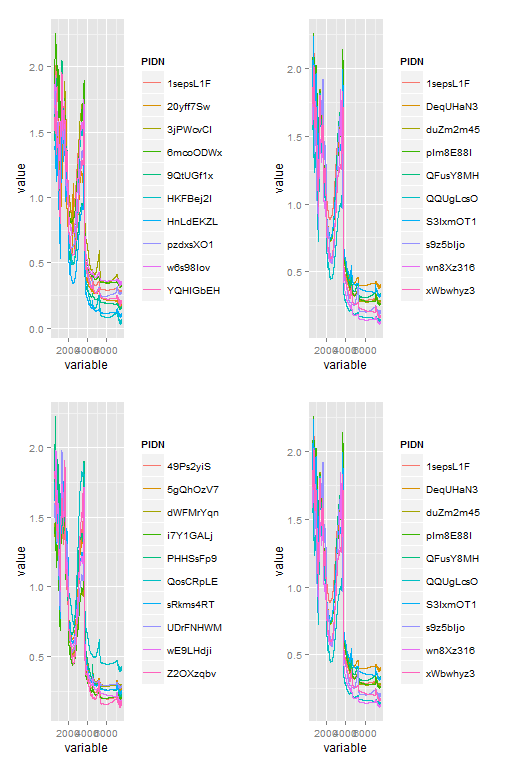
\includegraphics[width=\textwidth]{Rplot.png}
	\caption{\label{fig:Rplot} Right: With CO2. Left: W/O CO2. Top: Topsoil. Below: Subsoil}
\end{figure}

\section{Preprocessing}
Visualization of data helped to see the existence of noise in the data. To remove the noise and smooth the signals the following techniques are used.
\begin{itemize}
\item Multiple Scatter Correction:

	Multiple Scatter Correction is a math treatment to correct the scatter in the spectra. The scatter is produced for different physical circumstances such as particle size and packaging. Normally scatter makes worse the correlation of the spectra with the constituent of interest.
	
	\item First Derivative Transformation:
	
	The goal of using the first derivative is not necessarily to create a transformed data set (or new variables), but rather to smooth out noise in the original spectra. In this project the method helped to:
	
	Reduce baseline offset
	
	Resolve absorption overlapping
	
	Enhance small spectral absorptions
\item Discrete Wavelet Transform Technique:

The discrete wavelet transform technique pairs the input values, storing the difference and passing the sum. This has a huge number of applications in science, engineering, mathematics and computer science. Most notably, it is used for signal coding, to represent a discrete signal in a more redundant form, often as a preconditioning for data compression. Practical applications can also be found in signal processing of accelerations for gait analysis, in digital communications and many others. 

\end{itemize}

\section{Review of Used Algorithms}
The performance of different methods was tested for calibrating reflectance spectra to SOC, pH, Ca, P, Sand. These techniques are partial least squares regression (PLSR), random forests (RF) , k – Nearest Neighbor, Support Vector Machines and Linear Regression.
\begin{itemize}
	\item Partial Least Squares Regression (PLSR)
	
	Partial least squares regression (PLS regression) is a statistical method that bears some relation to principal components regression; instead of finding hyperplanes of minimum variance between the response and independent variables, it finds a linear regression model by projecting the predicted variables and the observable variables to a new space. Because both the X and Y data are projected to new spaces, the PLS family of methods are known as bilinear factor models. Partial least squares Discriminant Analysis (PLS--DA) is a variant used when the Y is categorical. 
	
	\item Random Forest (rf)
	
	In random forests each tree in the ensemble is built from a sample drawn with replacement (i.e., a bootstrap sample) from the training set. In addition, when splitting a node during the construction of the tree, the split that is chosen is no longer the best split among all features. Instead, the split that is picked is the best split among a random subset of the features.
	
	\item k--Nearest Neighbor (k--NN)
	
	Neighbors-based classification is a type of instance-based learning or non-generalizing learning: it does not attempt to construct a general internal model, but simply stores instances of the training data. Classification is computed from a simple majority vote of the nearest neighbors of each point: a query point is assigned the data class which has the most representatives within the nearest neighbors of the point.
	
	\item Support Vector Machines (SVM)
	
	In machine learning, support vector machines (SVMs, also support vector networks) are supervised learning models with associated learning algorithms that analyze data and recognize patterns, used for classification and regression analysis. Given a set of training examples, each marked as belonging to one of two categories, an SVM training algorithm builds a model that assigns new examples into one category or the other, making it a non-probabilistic binary linear classifier. An SVM model is a representation of the examples as points in space, mapped so that the examples of the separate categories are divided by a clear gap that is as wide as possible. New examples are then mapped into that same space and predicted to belong to a category based on which side of the gap they fall on.
	
	\item Linear Regression (lm)
	
	In statistics, linear regression is an approach for modeling the relationship between a scalar dependent variable y and one or more explanatory variables denoted X. The case of one explanatory variable is called simple linear regression. For more than one explanatory variable, the process is called multiple linear regression. In linear regression, data are modeled using linear predictor functions, and unknown model parameters are estimated from the data. 
	
\end{itemize}

\section{Implementing the Algorithms}

Before making any model we used PCA to reduce the dimensions of the data. Principal component analysis (PCA) is a statistical procedure that uses an orthogonal transformation to convert a set of observations of possibly correlated variables into a set of values of linearly uncorrelated variables called principal components. The number of principal components is less than or equal to the number of original variables. This transformation is defined in such a way that the first principal component has the largest possible variance (that is, accounts for as much of the variability in the data as possible), and each succeeding component in turn has the highest variance possible under the constraint that it is orthogonal to (i.e., uncorrelated with) the preceding components.

In next step we used the following R libraries to call the required functions for training and prediction. 

\begin{itemize}
	\item RWeka - Used for PCA
	\item Wavelets - Used for Discrete wavelet transformation
	\item caret - Used for training and predicting the model
	\item pls - Used for training model with partial least squares
	\item kernlab - Used for training model with SVM
	\item randomForest - Used for training model with rf
\end{itemize}

\section{Algorithm Comparison}
The root-mean-square error (RMSE) is a frequently used measure of the differences between value predicted by a model or an estimator and the values actually observed. Basically, the RMSE represents the sample standard deviation of the differences between predicted values and observed values.

$$RMSE = \sqrt{\frac{1}{n}
	\sum_{j=1}^{n}(y_j-\hat{y_j})^2}$$



Figure1 includes the RMSE values gained for each response variable using different models. The best model for predicting each of 5 response variable is the one with the lowest RMSE value.

\begin{figure}[h!]
	\centering
	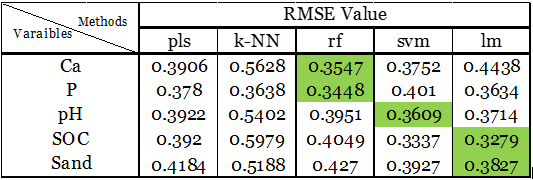
\includegraphics[height= 4cm,width=10cm]{Table.png}
	\caption{\label{fig:Table} Comparison of RMSE of each model for each response variable}
\end{figure}

\subsection{Software Used}
Used RStudio Version 0.98.1028 - 2009 --2013 RStudio, Inc.\\

System Configuration - 
\begin{itemize}
	\item Intel(R) Core(TM) i5-3337U
	\item 4.00 GB RAM
	\item 64- bit Operating System, x64-based processor
	\item Windows 8.1
\end{itemize}

The code is attached with the document with comments explaining all the steps.
\newpage
\section{Conclusion}

The best models for predicting response variables are:\\

\noindent Ca  - Random Forest\\
P – Random Forest\\
pH – Support vector machines \\
SOC – Linear regression\\
Sand – Linear regression \\

\newpage
\bibliography{document}
\bibliographystyle{abbrvnat}

\end{document}